\chapter{In litterae}

\section{Trwałość amidów}

\begin{marginfigure}[7\baselineskip]
  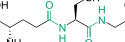
\includegraphics{schemes/glutathione}
  \caption{
    Glutation --- trójpeptyd o właściwościach przeciwulteniających,
    z wiązaniami amidowymi zanaczonumi na zielono.
  }
  \label{fig:glutathione}
\end{marginfigure}
Wiązanie amidowe występuje w naturze niezwykle powszechnie.
Można nawet pokusić się o stwierdzenie, że jest ono jednym z budulców życia ---
w końcu peptydy, podstawowa struktura biocheniczna złożonych organizmów,
to łańcuchy aminowkasów, połączonych wiązaniami amidowymi.
Za przykład posłużyć może glutation --- trójpeptyd o właściwościach przeciwulteniających,
występujący powszechnie w organizmach roślinnych i zwierzęcych\autocite{wu04},
przedstawiony na \cref{fig:glutathione}.
  
\begin{marginfigure}
  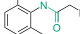
\includegraphics{schemes/lidocaine}
  \caption{
    Lidokaina --- przykład leku posiadającego ugrupowanie amidowe
    (zaznaczone na zielono).
  }
  \label{fig:lidocaine}
\end{marginfigure}
Ugrupowanie to można też znaleźć w wielu związkach biologicznie czynnych.
Za prosty przykład niech posłuży lidokaina, przedstawiona na \cref{fig:lidocaine},
powszechnie stosowana jako środek miejscowo znieczulający.
Przykładów takich możnaby przytoczyć wiele, bo jak pokazuje analiza produkcji farmaceutyków,
\SI{66}{\percent} leków syntezuje się tworząc wiązanie amidowe\autocite{carey06}.

W latach 30. ubiegłego wieku firma DuPont wprowadziła na rynek poliamidy na rynek tworzyw sztucznych pod nazwą handlową Nylon.
Ten bardzo trwały materiał szybko znalazł zastosowanie w wielu gałęziach przemysłu.
Stosuje się go przede wszystkim do wytwarzania syntetycznych włókien tekstylnych,
ale też do produkcji szczoteczek do zębów, strun do instrumentów, żyłek wędkarskich, czy opakowań żywności.


Tę powszechność --- zarówno wśród produktów naturalnych, jak i wytworów cywilizacji ---
amidy zawdzięczają między innymi swojej wyjątkowo niskiej reaktywności.
Wiązanie amidowe ulega niewielu przemianom chemicznym, a jeśli już, to 
zwykle wymaga stosowania bardzo ostrych warunków prowadzenia reakcji.
Ta niezwykła trwałosć wynika z bardzo efentywnego nakładania się orbitali 
molekularnych atomu azotu oraz $\pi$ wiązania podwójnego \ch{C=O}.
Pozwala to na wydajną delokalizację elektronów w obrębie wiązania i znaczny 
udział dwóch możliwych struktur zwiterionowych, jak widać na \cref{sch:resonance}.
\begin{scheme}
  \centering
  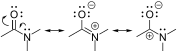
\includegraphics{schemes/resonance}
  \caption{
    Struktury rezonansowe wiązania amidowego, zapewniające mu niezwykłą trwałość.
  }
  \label{sch:resonance}
\end{scheme}


\section{Prezkształcenia amidów}
Przez długi czas chemia amidów była raczej uboga ---
ograniczała się przede wszystkim do prostych reakcji, dziś uznanych za podręcznikowe.
W pierwszej kolejności można wymienić ich redukcję do amin oraz hydrolizę.

\section{Odczynnik Schwartza}
